\subsection{Surface Reconstruction}
\todourgent[author=Benni,inline]{Move this section into appendix! Only the weak spot surface reconstruction should be named. Alternatives, see appendix}
Our implementation of the surface reconstruction scheme explained in \autoref{ssec:reconstruction} and the two-scale approach described in \autoref{ssec:parametrization} yet only works for very simple structures like spheres or tori. For more complicated structures -- for example the output of a topology optimization tool -- we either have to use a very high resolution, or we have to apply certain optimizations, which will be explained in the following.

\subsubsection{More flexible Dual Contouring}
Our implementation of \ac{DC} is a very basic one. But this causes problems, when it comes to the coarse resolution of our two scale approach: We need an as coarse as possible mesh, which has the same topology as our fine mesh. These goals cannot be reached with a basic approach, but only with an adaptive and topology safe \ac{DC} algorithm like described in \cite{Hermite2002}.

\subsubsection{Dual Marching Methods}
The non-manifold edges generated by \ac{DC} have been resolved by applying a remeshing scheme. But there are also hybrid methods of \ac{DC} and \ac{MC}, which have been developed in order to come up with the drawbacks. These methods use ideas from both the \ac{MC} and the \ac{DC} approaches (For a short summary of those ideas see \autoref{tab:dualmarching}). Using one of these methods would be a way of avoiding non-manifold edges from the beginning while keeping all the beneficial properties of \ac{DC}.
\begin{table}[H]
\begin{tabularx}{\textwidth}{X|X}
\multicolumn{1}{c|}{\acl{MC}} 
    & \multicolumn{1}{c}{\acl{DC}} 
\\
\hline
\begin{itemize}[ topsep = 0pt, leftmargin=1em]
\item traverse voxels and use a look up table for the creation of faces
\item creates manifold and ambiguity free surfaces
\end{itemize}
&
\begin{itemize}[ topsep = 0pt, leftmargin=1em]
\item place vertices inside voxel\footnote{Determine positions by -- for example -- minimizing \autoref{eq:QEF}.}
\item construct \acp{quad} by joining vertices in voxels with a common edge
\end{itemize}
\end{tabularx}
\caption{ideas from \ac{DC} and \ac{MC} contributing to dual marching methods.}
\label{tab:dualmarching}
\end{table}
In the following we will briefly introduce two of those hybrid methods:

\begin{itemize}
\item \textbf{\acl{DualMC}}:
The \acf{DualMC} method is --- like already stated above --- a hybrid of \ac{MC} and \ac{DC}: We traverse the cubes like in \ac{MC} and insert vertices and connect them like in \ac{DC}. The combination of the $256$ different cases from the basic \ac{MC}, the extension for creating ambiguity free surfaces and the framework of \ac{DC} results in a very effective but also complex algorithm. A drawback of this method is that for certain configurations we have to create non-\ac{quad} faces --- especially faces with odd number of vertices are difficult to convert to \acp{quad}, if one wants to obtain a \ac{quad}-only surface like in \ac{DC}. We refer the interested reader to  \cite{Nielson2004, Zhang2012}.

\item \textbf{\acl{DualMT}}:
While \ac{DualMC} is a very complicated algorithm, \acf{DualMT} uses tetrahedra instead of cubes and therefore reduces the $256$\footnote{With a proper treatment of ambiguities we get even more than those $256$ cases.} different cases from \ac{MC} to $2^4=16$ cases. Furthermore a treatment of ambiguous cases is not necessary anymore, since there are no ambiguous cases for this method\todointern{really? check this or find reference!}.
Even though the method is working on tetrahedra, we can still apply it to a voxel dataset, by composing each cube out of 5 or 6 tetrahedra (\autoref{fig:splittingCubes}). Nevertheless, this high amount of simplification comes with a drawback: The treatment of ambiguous cases depends on the splitting scheme applied to a cube\todointern{proof or reference! Show 2D example.}. Further detail on this method can be found in \cite{Nielson2008}.

\begin{figure}
\begin{center}
\begin{subfigure}[t]{.45\textwidth}
\begin{center}
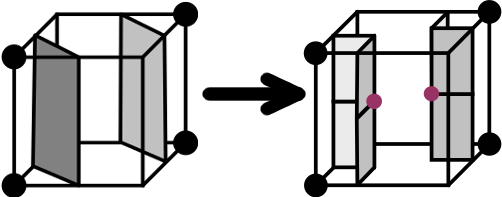
\includegraphics[width = .8\textwidth]{Pictures/SurfaceReconstruction/MCtoDualMC.png}
\subcaption{How one of the \ac{MC} cases is treaten in \ac{DualMC} algorithm (figure from \cite{Nielson2004})}
\end{center}
\end{subfigure}
\hfill
\begin{subfigure}[t]{.45\textwidth}
\begin{center}
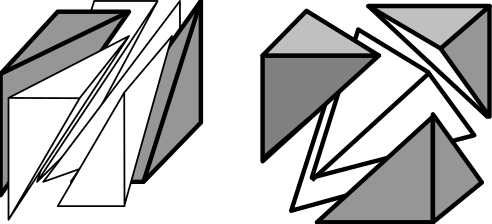
\includegraphics[width = .8\textwidth]{Pictures/SurfaceReconstruction/SplittingCubes.png}
\caption{Two different subdivision schemes for cubes into tetrahedra (figure from \cite{Nielson2008})}
\label{fig:splittingCubes}
\end{center}
\end{subfigure}
\end{center}
\end{figure}

\end{itemize}
